\chapter{Disjuctive Interconnection Graphs for Disease Gene Prioritization}
\label{chap:digi}
\section{Motivation}
Disease-gene association recovery is a major goal in molecular biology and medical that has received much attention from many researchers. As a consequence, a big progress has been made in the last decade. Concerning a genetic disease, there normally a small number of genes known to be related to it. In order to find out the complement set of the known disease gene set, one way is to search for whole genome or specific regions that often contain a large number of suspected genes (candidate genes). It is obvious not a good idea as it is expensive not only in term of time consuming but also from financial aspect. For this reason, a considerable number of \textit{gene prioritization} methods have been proposed. A gene prioritization method aims at ordering candidate genes from the most to the least probable to be associated to the disease. The top genes in the ranking are then sent to biologists and medical scientists for further studies to determine whether each gene is related to considered disease.

Genetics data are growing at a fast pace thanks to the development of High-throughput technologies. Different data sources are made available in which each data source focuses on a specific aspect of genes. Therefore, only integration of different heterogeneous data sources is supposed to lead to high performance of gene inference systems. It is due to combining sources brings more unified views about genes. Graphs are known the best data structures for genetic data where gene relations are encoded as links. So the data integration can now turn to graph integration. 

One of the key points which determins the performance of machine learning systems is the definition of the entity similarity, graph node similarity in our case. Kernel is well-known as a universal paradigm used to capture similarity between entities any any kind of form. Thus, many graph node kernels are proposed to measure similarity between graph nodes and applied to graph-based data integration systems solving for disease gene prioritization. However, most methods/systems are based on multiple kernel learning that first compute kernel for each graph separately and then try to learn a final normally based on a data driven way. It shows a disadvantage since data driven only can impact to graph unit level or all nodes (genes) in a graph are assigned a same weight when combining. 

In this paper, we first propose a novel graph integration which allows genes not only linked with genes in the same graph but also are able to be linked with genes from all other graphs. We then employ a relevant compositional graph kernel named conjuctive disjuctive graph node kernel (CDNK).

\section{Related work}
In the last decade, there is a number of gene prioritization methods which are based on data integration have been proposed. They can be classified into two groups by considering their integration stage.

The first group contains methods that first separately define the similarities between genes from each data source. They then combine these obtained similarities to have the final gene similarities.

\cite{epu} proposed a method named EPU which is a modification of PUDI \cite{pudi}. Unlike most other methods that treat unknown genes homogeneously, in EPU, for each data source, the unknown gene set is partitioned into multiple positive and negative sets with different confidence scores (weights). It then employs an ensemble procedure to compute the final weight for unweighted genes in the unlabelled set. Besides, three weighted classifiers are applied. Finally, ensamble PU learning is used to decide whether an unlabelled gene belongs to positive or negative set. Experiments show that EPU gets significantly higher performance compared to many methods.

\cite{dir} proposed a candidate gene prioritization approach, DIR, that can integrate multiple data sources by taking advantage of a unified graphic representation of information. DIR employs a diffusion kernel to define a global similarity for all pairs of genes in every source. Later it defines a data integration rank score to select the most informative evidence among a set of data sources.

ProDiGe (\cite{prodige}) is an efficient method that uses MKL to combine data sources [8]. The global similarity between genes are computed by using the inner product between feature vectors and a diffusion kernel for PPI. Then a MKL algorithm is used to combine pre-defined kernels and learn an optimal kernel. Next, it uses a biased SVM to identify potential gene-disease associations. In ProDiGe, the set of data sources can be expanded easily. However, the use of a single kernel type and the employed MKL algorithm could be considered as limitations.

\cite{mrf} a kernel-based Markov random field algorithm is proposed. In this method, graph kernels are used to define global similarity between genes. From a prior probability vector, MRF algorithm computes the posterior probability vector. This vector gives the probability of each candidate gene to be related to the considered disease. The use of an adaptation of the Gibbs sampling procedure allows to assign weights for different data sources. MRF method is flexible in terms of data integration and it outperforms other previous methods that use Markov random field. However, during the Gibbs sampling process, it takes a long time in order to maintain a long Markov chain for every gene. 

A method proposed in \cite{f3pc}, notated as F3PC, shows better results compared with many disease gene prioritization tools. The strength of this method is the use of modified conditional random field model, that simultaneously utilizes both gene annotations and gene interactions while preserving their original representation. 

\cite{scuba} introduced a scalable kernel-based method for gene prioritization in which an efficient of multiple kernel learning is proposed to find an optimal kernel given a set of predefined ones. Scuba can deal with a high number of data sources with a linear time complexity w.r.t number of sources and a constant memory consumption.

The second group includes algorithms that merge graphs derived from different sources to form a single one. It then computes gene similarities underlying the achieved graph.

\cite{rwr} introduces a method named RWR that merges different networks into a single one. Then a global similarity measure, the random walk with restart algorithm, is applied to rank the candidate genes. This method often shows better performance compared to some other methods in terms of prediction accuracy and time consumption. Although it integrates useful information from different data sources, it also integrates noise and it does not take the individual weight of sources into account.

In order to facilitate for users, some methods for disease gene prioritization are made available as web tools such as Suspects \cite{suspect}, ToppGene \cite{toppgene}, GeneDistiller \cite{genedistiller}, GeneWanderer \cite{genewanderer}, Posmed \cite{posmed}, Candid \cite{candid}, Endeavour \cite{endeavour} and Pinta \cite{pinta}. In \cite{unbiased_evaluation}, many web tools are described and evaluated. 

Regarding first group, the similarities of nodes are computed separately from different graphs. They are then combined by assigning a weight for each source. It means, every nodes in a same graph are assigned with a same weight. Therefore, it is not able to distingush the impact level of different genes on a considered disease. The fact is that some genes are more relevant the the disease (task) than others. For the second group, graphs are combined before a single similarity measure is carried out. In this case, methods cannot effectively take the advantage from the use of multiple graphs since the properties of individual graphs could not be preserved.

In this paper, we propose a method that can overcome the aboved analysed limitations from these two groups. More specifying, by proposing a novel paradigm for graph integration and employing a logical, effective node kernel, in our method the features of a node in a graph are extracted from not only in the graph it is placed, but also from other graphs. Therefore, it preserves the characteristics of single graphs in the one hand and it allows genes in a graphs to have different weights when combining for the final similarities on the other hand. We show the outperformance of our method comparing with other methods in two different setting.
\section{Method}
In this section, we first introduce definitions and notations used for the rest of the paper. We then describe our proposed method for disease gene prioritization.

\subsection{Background, definition and notations}
A graph is a structure notated as $G=(V,E)$ where $V$ is the set of nodes and $E$ is the set of links. We define the \textit{distance} $\mathcal{D}(u,v)$ between two nodes $u$ and $v$, as the number of edges on the shortest path between them. The \textit{neighborhood} of a node $u$ with radius $r$, $N_r(u) = \lbrace v\ |\ \mathcal{D}(u,v) \leq r \rbrace$, is the set of nodes at distance no greater than $r$ from $u$. The corresponding \textit{neighborhood subgraph} $\mathcal{N}_{r}^{u}$ is the  subgraph induced by the neighborhood (i.e. considering all the edges with endpoints in $N_r(u)$). The \textit{degree} of a node $u$, $deg(u) = |\mathcal{N}_{1}^{u}|$, is the cardinality of its \textit{neighborhood}. The maximum node degree in the graph $G$ is $deg(G)$.

\textbf{Disease gene prioritization:} Let us consider a set of genes $\mathcal{G} = \lbrace g_1, g_2, \ldots, g_N \rbrace$ that represents either the global set of genes in the genome or a subset of it. Given another set $\mathcal{P} = \lbrace g_1, g_2, \ldots, g_m \rbrace, \, \mathcal{P} \subset \mathcal{G}$ containing genes known to be associated to a genetic disease, gene prioritization is the task that aims to rank genes in the set of candidates $\mathcal{U} = \mathcal{G} \setminus \mathcal{P}$ according to their likelihood of being related to that disease.

\textbf{The Conjunctive Disjunctive Node Kernel:} In \cite{cdnk}, a modification of NSPDK kernel \cite{nspdk} named CDNK is proposed to define the similarity for graph nodes. CDNK defines a node kernel $K(G_u,G_{u'})$ between two copies of the same network $G$ where it distinguishes the nodes $u$ and $u'$ respectively. This kernel extracts subset of NSPDK features whose $u$ as one of the roots and uses as features for $u$. Interestingly, it distingushes between between two types of edges, called {\em conjunctive} and {\em disjunctive} edges. Hence, it is relevant to apply on graphs resulted from the network decomposition presented in \ref{network-decomposition}. Regarding the edge types, it considers conjunctive edges only when computing distances to induce neighborhood subgraphs. When choosing the pair of neighborhoods to form a single feature, it additionally considers roots $u$ and $v$ that are not at distance $d$ but such that $u$ is connected to $w$ via a disjunctive edge and such that $w$ is at distance $d$ from $v$. In this way disjunctive edges can still allow an {\em information flow} even if their endpoints are only considered in a pairwise fashion and not jointly. 

\begin{figure}[ht]
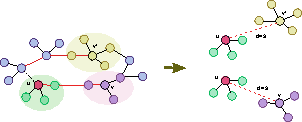
\includegraphics[width=0.9\columnwidth, height=4cm]{img/cdnk.pdf}
\caption{CDNK}
\label{fig:01}
\end{figure}

Formally, It defines two relations: the \textit{conjunctive relation} $R^{\wedge}_{r,d}(A_u, B_v, G_u)$ identical to the NSPDK relation $R_{r,d}(A_u, B_v, G)$,  and (ii) $\mathcal{D}(u,v)= d$; the \textit{disjunctive relation} $R_{r,d}^{\vee}(A_u, B_v, G_u)$ is true {\em iff} (i)  $A_u \cong \mathcal{N}_r^u$ and $B_v \cong \mathcal{N}_r^u$ are true, (ii) $\exists w$ s.t. $\mathcal{D}(w,v)= d$, and (iii) $(u,w)$ is a disjunctive edge. Besides, it defines $\kappa_{r,d}$ on the  inverse relations ${R^{\wedge}_{r,d}}^{ -1}$ and ${R^{\vee}_{r,d}}^{ -1}$ \vspace{8pt}\\

 $\kappa_{r,d}(G_u,G_{u'}) = \!\!\!\!\!\!\!\!\!\!\!\!
 \sum\limits_{\substack {A_u,{B}_{v} \in {R_{r,d}^{\wedge}}^{ -1}(G_u) \\ A'_{u'},{B'}_{v'} \in {R_{r,d}^{\wedge}}^{ -1}(G_{u'}) }} \!\!\!\!\!\!\!\!\!\!\!\!
  { \textbf{1}_{A_u \cong A'_{u'}} \cdot { \textbf{1}_{B_{v} \cong B'_{v'}}}}
+ \!\!\!\!\!\!\!\!\!\!\!\! \\
 \sum\limits_{\substack {A_u,{B}_{v} \in {R_{r,d}^{\vee}}^{ -1}(G_u) \\
  A'_{u'},{B'}_{v'} \in \ {R_{r,d}^{\vee}}^{ -1}(G_{u'}) }} \!\!\!\!\!\!\!\!\!\!\!\!
  { \textbf{1}_{A_u \cong A'_{u'}} \cdot { \textbf{1}_{B_{v} \cong B'_{v'}}}}
  $. \vspace{8pt}\\
The CDNK is finally defined as $K(G_u,G_v) = \sum\limits_{r}{\sum\limits_{d}{\kappa_{r,d}(G_u,G_v)}}$, where once again for efficiency reasons, the values of $r$ and $d$ are upper bounded to a given maximal $r^*$ and $d^*$.
\subsection{Disjunctive interconnection graph integration}
In this section, we first introduce the flow of our proposed method for disease gene prioritization. We then describe each part in detail.

We consider a set of graphs $\mathcal{G} = \lbrace g_1, g_,\ldots, g_n \rbrace$ where we refer each graph as a layer. Our method consists of following steps:
\begin{itemize}
\item Graph decomposition: Each graph is transformed into a collection of sparse sub-networks.
\item Graph labeling: Different ways are introduced to label for node and edges of each graph.
\item Graph union: we connect the set of graphs obtained from previous steps to form a single graph whose layers are linked with disjunctive links.
\item Similarity definition: we apply a particular graph node kernel, CDNK \cite{cdnk},  on the union graph to define node similarities which will be fed into a kernel machine to construct a model for disease gene inference.
\end{itemize} 

\begin{figure}[ht]
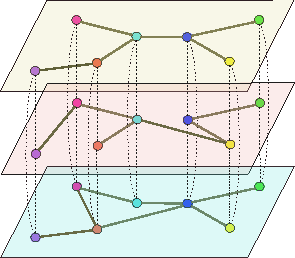
\includegraphics[width=0.9\columnwidth, height=6cm]{img/multilayers.pdf}
\caption{Graph Disjunctive Interconnection Illustration}
\label{fig:graph_interconnection}
\end{figure}

\subsection*{Graph Decomposition} 
\label{network-decomposition}
Graph decompositional kernels can only efficiently work on graphs whose nodes with low degree. However, it is common to find nodes with degree in gene-based networks. It prevents decompositional kernels from showing promising performance due to the high number of neighborhood subgraphs. To overcome this problem, in \cite{cdnk}, a network decomposition procedure is proposed with the aim of transforming a given network into a collection of sparse sub-networks whose \textit{conjunctive} links only are linked by \textit{disjunctive} links. The decompostion works by first applying the k-core decomposition iteratively and then the clique decomposition. Following we describe in detail each decomposition type in detail.

\textit{Iterative k-core decomposition}: The node set is partitioned in two groups on the basis of the degree of each node w.r.t. a threshold degree $D$. The node partition is used to induce the conjunctive vs disjunctive edge partition: edges that have endpoints in the same part are marked as conjunctive, while edges with endpoints in different parts are marked as disjunctive. We apply the k-core decomposition iteratively considering only the graph induced by the conjunctive edges until no node has a degree \footnote{The degree is defined by only considering incident conjunctive edges.}greater than $D$.

\begin{figure}[ht]
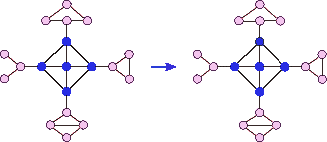
\includegraphics[width=0.9\columnwidth, height=3cm]{img/k_core.pdf}
\caption{K-core decomposition}
\label{fig:01}
\end{figure}

\textit{Clique decomposition}: To model the notion that nodes in a clique are tightly related, we summarize the whole clique with a new 'representative' node. All the cliques (completely connected subgraphs) with a number of nodes greater than a threshold size $C$ are identified. The endpoints of all edges incident on the clique's nodes are transferred to the representative node. Disjunctive edges are introduced to connect each node in the clique to the representative. Finally all edges with both endpoints in the clique are removed.
\begin{figure}[ht]
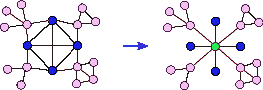
\includegraphics[width=0.9\columnwidth, height=2.5cm]{img/cliques.pdf}
\caption{Clique decomposition}
\label{fig:01}
\end{figure}
In our work a network is transformed by applying first the iterative k-core decomposition and then the clique decomposition.

\subsection*{Graph labeling}
\textbf{Node labeling}: we employ two methods to label for nodes in a graph. Both methods are based on the idea that genes with similar number of neighborhoods tend to have similar properties. We consider both conjunctive and disjunctive edges to compute the node degree.
\begin{itemize}
\item The first node labeling function, $\ell_1$, assigns the degree for nodes $u$ having degree less than or equal a user defined threshold $T$ ($T=5$ in our experimental evaluation). However degree values larger than $T$ are subsequently discretized into $k$ levels. Formally, the labeling function is defined as:
\begin{center}
$\ell_1(u) = \left\{
	\begin{array}{ll}
		deg(u),\  & \mbox{if } deg(u) \leq T \\
		T+i,\ & \mbox{if } deg(u) > T
	\end{array}
\right.$,
\end{center}
where $i = \lceil \frac{deg(u)-T}{bin}\rceil$, $bin = \frac{deg(G)-T}{\lambda - T}$ and $\lambda$ ($\lambda > T$) is the maximum number of symbols used. The value of $\lambda$ depends on the degree distribution and can be tuned as a hyperparameter of the approach.

\item The second node labeling function, $\ell_2$ implements the idea of equal frequency discretization. Given number of bins, $k$, we assign nodes into bins such that two criteria. First, nodes with similar degree are assigned into the same bin. Second, every bin needs to have similar number of nodes. We then use the bin ID as label for its nodes.
\end{itemize}

\noindent \textbf{Edge labeling}: We assign labels for every edges in a layer as its layer ID.

\subsection*{Graph union} 
Consider a layer tuple $g_i$, $g_j$ ($g_i, g_j \in \mathcal{G}$) and two nodes $u\in g_i,\ v \in g_j$ such that $u$ and $v$ are both represent for a same gene, we connect $u$ and $v$ by a disjuctive link. As the consequence, we achieve a graph $g$ whose nodes represeting same genes in all graph layers are linked by disjuctive links. Figure \ref{fig:graph_interconnection} is a visualization for our graph integration idea. 

\subsection*{Similarity definition}
We employ CDNK to define similarity for the similarity for any couple of genes. The similarity between two genes $g_i$ and $g_j$ is the summation of similarity of between their corresponding nodes on all layers.
\section{Experiments}
In order to evaluate the performance of our proposed method, we conduct two separate experiments. In the first experiment, \textit{cross-validation evaluation}, we desire to compare our method with state-of-the-are methods for disease gene prioritization in the first experiment, while we intend to compare the performance our proposed method with web-tools for disease gene identification in the second experiment, \textit{unbiased evaluation}. Following, we first describe data sources employed for our experiments, we then present the procedures to carry out them.

\subsection*{Data sources}
\begin{itemize}
	\item \textbf{Human Protein Reference Database} (\textbf{HPRD}): a database of curated proteomic information pertaining to human proteins. It is derived from \cite{hprd1} with 9,465 vertices and 37,039 edges. We employ the HPRD version used in \cite{hprd2} that contains 7311 nodes and 30503 edges. 	
	
	\item \textbf{BioGPS} \cite{biogps1, biogps2} a gene co-expression graph (7311 nodes and 911294 edges) constructed from the BioGPS dataset, which contains 79 tissues, measured with
the Affymetrix U133A array. Edges are inserted when the pairwise Pearson
correlation coefficient (PCC) between genes is larger than 0.5.	
	
	\item \textbf{Pathways}: Pathway datasets are obtained from the database of KEGG \cite{kegg}, Reactome \cite{reactome}, PharmGKB \cite{pharmgkb} and PID \cite{pid}, which contain 280, 1469, 99 and 2679 pathways, respectively. A pathway co-participation network is constructed by connecting genes that co-participate in any pathway.
	\item \textbf{String}: The String database gathers protein information covering seven levels of evidence: genomic proximity in procaryotes, fused genes, co-occurrence in organisms, co-expression, experimentally validated physical interactions, external databases and text mining. Overall, these aspects focus on functional relationships that can be seen as edges of a weighted graph, where the weight is given by the reliability of that relationship. To perform the unbiased evaluation we employed the version 8.2 of String \cite{string}, from which we extracted functional links among 17078 human genes.
	\item \textbf{Omim}: OMIM is a public database of disease-gene association. Genes
implicated in the same disease are more likely to be involved in other
similar diseases as well. Therefore, Omim network is formed by connecting genes which are involved in common disease(s).
\end{itemize}

\subsection*{Cross-validation evaluation} We follow the experimental setting used in \cite{f3pc}. In this experiment, three datasets are employed: BioGPS, HPRD and Pathways. To perform the experiment, 12 disease-gene associations are selected from OMIM data source with at least 30 confirmed genes. Concerning each disease, we construct a a positive set ($P$) which contains its all confirmed disease genes. For the negative set ($N$), we randomly sample from the set of genes which are related to at least one disease, but not with the disease that defines $P$, such that $|N| = \frac{1}{2}|P|$. 

For evaluation, a leave-one-out cross validation is used. Iteratively, each turn a gene in the training set ($P \cup N$) is selected to be the test gene and the remaining genes used to train the model. For each test gene $g_i$, the model returns a score $s_i$ proportional to the likelihood of being associated to the disease. Next a decision score $q_i$ is
computed as the top percentage value of $s_i$ among all candidate gene scores.
We collect all decision scores for every test genes to compute the area under
the curve for the receiver operating characteristic (AUC-ROC).

\subsection*{Unbiased evaluation} When a new gene-based discovery is made, most related data sources are updated. Therefore, the performance of methods evaluated through the previous experiment could be over-optimistic. To void this inflation, we conduct our experiment following the setting used in \cite{unbiased_evaluation} with the aim at comparing our method performance with different web tools for disease gene prioritization.
Newly discovered disease-gene associations were collected over a timespan of six months, gathering 42 associations. As soon as a new association was discovered, eight pre-selected gene prioritization web tools were queried with a proper training set in order to mimic the discovery through each of them. These 42 predictions were used to assess the ability of the tools to successfully prioritize disease genes. The idea behind this procedure is to anticipate the integration of the associations in the data sources and so avoid biased predictions.

To evaluate the performance of DIGI, we backdated our datasets to a time prior to May 15, 2010 by employing String v8.2 data \cite{string} and OMIM. The candidate sets were constructed by considering all genes with Ensembl \cite{ensembl} gene identifier within the chromosomal regions around the test genes, in order to get on average 100 candidates for each trial. Then, we performed prioritizations for each test gene in two distinct cases - genome-wide and candidate set-based prioritizations. In genome-wide prioritizations all coding genes in the genome were prioritized, while in candidate set-based tests only the genes belonging to the candidate groups were ranked. In both cases, we normalized ranking positions over the total number of genes in order to get the median and the standard deviation of the normalized ranks for test genes. We also computed the true positive rate (TPR) relatively to some representative thresholds (5\%, 10\% and 30\% of the ranking) and the AUC obtained by averaging over the 42 prioritizations.

\subsection*{Model Selection} The hyper-parameters of our method are set using a 3-fold on training set in which one fold is used for training the model and two remaining folds are used for validation. For CDNK, we try for the degree threshold value in $\lbrace 10,\ 15,\ 20 \rbrace$, clique size threshold in $\lbrace 4,\ 5 \rbrace$, maximum radius in $\lbrace 1,\ 2 \rbrace$, maximum distance in $\lbrace 2,\ 3,\ 4 \rbrace$. The number of bins, $k$, in node labling function $\ell_1$ and $\ell_2$ is set in $\lbrace 7, 10, 12 \rbrace$. Finally, the regularization tradeoff $C$ for the SVM is chosen in $\lbrace 10^{-4}, 10^{-3}, 10^{-2},\ 10^{-1}, 1,\ 10,\ 10^2, \\ 10^3,\ 10^4 \rbrace$.
\section{Results and discussion}
Table \ref{tab:unbiased_evalutation} and \ref{tab:cross_validation_evaluation} show the performance of our proposed method together with different methods and tools in unbiased evaluation and cross validation setting, respectively. Overall, DIGI outperforms all compared methods. 

In the Unbiased evaluation setting, it can be seen from the table \ref{tab:unbiased_evalutation} that our method shows impressive performance which considerably higher than other's in both cases: Genome-wide and candidate genes. In particular, It shows big difference with the second best one, Scuba, with around 15$\%$ higher in both top 5$\%$ and 10$\%$. For the time and finance constraints, we normally take genes at very top in the ranking to have further tests. Therefore, having high accuracy in top 5$\%$ and 10$\%$ is really meaningful in practice.
It is also competive in top 30$\%$ with 85.7$\%$ and 88.1$\%$ for Genome-Wide and Candidate-Genes, respectively. It only shows a bit lower, around 2$\%$, than Endeavour with 90.5$\%$ in Candidate-Genes. Similarly for AUC measure, it show the best results in both cases with 87 and 86. Concerning the median rank, a huge gap between our method and the rest of compared methods can be observed from the table. We also report the relative position over 42 genes in the rank of DIGI in Figure \ref{fig:histogram-genomewide} and \ref{fig:histogram-candidate} in the two cases.
We can see that most test genes are ranked in the top of the rank, especially 22 and 17 genes are in in top 5$\%$ with 22 and 17 genes for Genome-Wide and Candidate, respectively. There is only 1 gene for each case in a very low position, top 80$\%$ and 90$\%$.


In the Cross validation setting, DIGI together with Scuba show the best performance with high gaps, at least 4.6$\%$ difference, compared with the rest of methods. Between DIGI and Scuba, DIGI presents a slightly higer than Scuba with 88.1$\%$ and 87.6$\%$, respectively. The worse performance methods in this setting are DIR and GeneWanderer.

\begin{table*}[!htb]
\caption{Performance of DIGI comparing with Scuba and other web tools on unbiased setting} 
\label{tab:unbiased_evalutation}
\setlength\tabcolsep{0pt} % let LaTeX compute intercolumn whitespace

\centering
\smallskip 
\begin{tabular*}{\textwidth}{@{\extracolsep{\fill}}ccccccl}
\hline
  Tool/Method & Response & Rank & TPR in top & TPR in top & TPR in top & AUC\\
              & rate (\%)    & median (\%) & 5\% (\%) & 10\% (\%) & 30\% (\%) & (\%)\\
\hline
Genome-Wide \\  
  DIGI & 100 & \textbf{4.73} & \textbf{52.4} & \textbf{59.5} & \textbf{85.7} & \textbf{87} \\
  Scuba & 100 & 10.55  &  33.3 & 47.6 & 78.6 & 80 \\
  Candid & 100 &  18.10 & 21.4 & 33.3 & 64.3 & 73 \\
  Endeavour & 100 &  15.49 & 28.6 & 38.1 & 71.4 & 79 \\  
  Pinta & 100 & 19.03 & 26.2 & 31.0 & 71.4 & 77 \\
  \hline
  Candidate-Genes \\
  DIGI & 100 & \textbf{6.10} & \textbf{50.0} & \textbf{59.5} & 88.1 & \textbf{86} \\ 
  Scuba & 100 &  12.95  &  28.6 & 45.2 & 73.8 & 78 \\
  Suspects & 88.9$^a$ &  12.77$^a$ & 33.3$^a$ & 33.3$^a$ & 63.0$^a$ & 76$^a$ \\
  ToppGene & 97.6 &  16.80 & 35.7 & 42.9 & 52.4 & 66 \\  
  GeneWanderer-RW & 88.1 &  22.10 & 16.7 & 26.2 & 61.9 & 71 \\
  Posmed-KS & 47.6 &  31.44 & 4.7 & 7.1 & 23.8 & 58 \\
  GeneDistiller & 97.6 &  11.11 & 26.2 & 47.6 & 78.6 & 85\\  
  Endeavour & 100 &  11.16 & 26.2 & 42.9 & \textbf{90.5} & 82 \\
  Pinta & 100 & 18.87 & 28.6 & 31.0 & 71.4 & 75 \\  
\hline
\end{tabular*}
\end{table*}
%====================================

\begin{figure*}
\centering
\begin{minipage}{.5\textwidth}
  \centering
  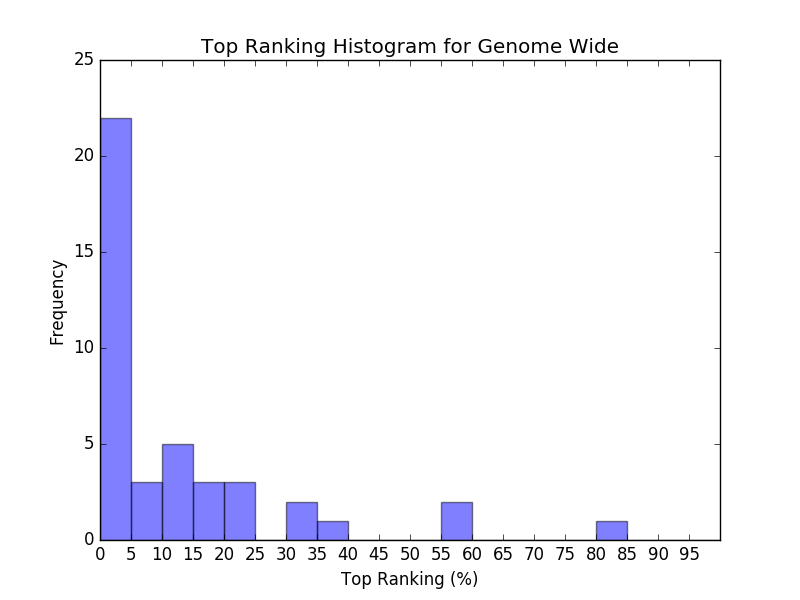
\includegraphics[width=1\linewidth]{img/histogram_genomewide.png}
  \caption{Top Rank Histogram for Genome-Wide Setting}
  \label{fig:histogram-candidate}
\end{minipage}%
\begin{minipage}{.5\textwidth}
  \centering
  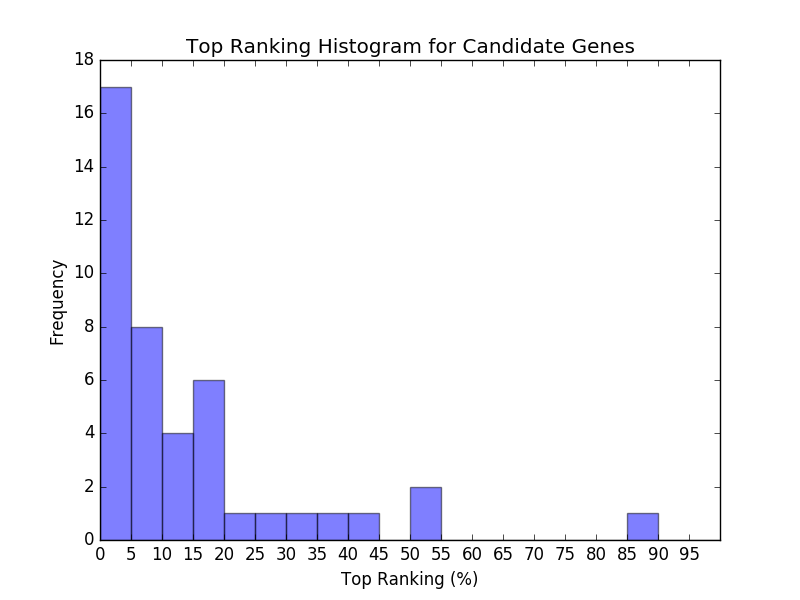
\includegraphics[width=1\linewidth]{img/histogram_candidate.png}
  \caption{Top Rank Histogram for Candidate Setting}
  \label{fig:histogram-candidate}
\end{minipage}
\end{figure*}



%====================================
\begin{table}[!htb]
%\setlength\tabcolsep{10pt} % let LaTeX compute intercolumn whitespace
%\centering
%\smallskip 
\caption{Performance of different methods on Cross validation setting} \label{tab:cross_validation_evaluation}
\centering
\begin{tabular}{cc}
\hline
  Method  & ROC-AUC (\%) \\
\hline
  DIR & 71.6 \\
  F3PC & 83.0 \\
  MRF & 73.1 \\
  GeneWanderer & 71.1 \\
  Scuba & 87.6 \\
 \textbf{DIGI} & \textbf{88.1} \\
\hline
\end{tabular}
\end{table}
\section{Conclusion}
We have proposed an efficient method for graph integration for disease gene prioritization. In our method, first graph layers are decomposed and disjunctively interconnected to let information traversing between layers. It then employ a perticular graph node kernel, which is able to efficiently exploit the graph structure resulted from the graph integration paradigm, to compute the capture the node similarities. As a consequence, it shows promissing performance and outforms all methods/tools employed in two experimental setttings.